\documentclass[12pt,oneside,a4paper,english]{article}
\usepackage[T1]{fontenc}
\usepackage[latin2]{inputenc}
\usepackage[margin=2.25cm,headheight=26pt,includeheadfoot]{geometry}

\usepackage{listings}
\usepackage{color}
\usepackage{titlesec}
\usepackage{titling}
\usepackage[framed, numbered]{matlab-prettifier}
\usepackage{changepage}
\usepackage{amsmath}
\usepackage{hyperref}
\usepackage{enumitem}
\usepackage{graphicx}
\usepackage{fancyhdr}
\usepackage{lastpage}
\usepackage{caption}
\usepackage{tocloft}
\usepackage{setspace}
\usepackage{multirow}
\usepackage{titling}
\usepackage{float}
\usepackage{comment}
\usepackage{booktabs}
\usepackage{indentfirst}
\usepackage{lscape}
\usepackage[english]{babel}
\usepackage{booktabs,caption}
\usepackage[flushleft]{threeparttable}
\usepackage[english]{nomencl}
\usepackage{xcolor}
\usepackage{lipsum}


% --- set footer and header ---
\pagestyle{fancy}
\fancyhf{}

\setlength{\parindent}{2em}
\title{Thesis} % to reference as \title, dont use \maketitle
\makeatletter\let\Title\@title\makeatother



\lstset{language=Matlab,
style=Matlab-editor,
basicstyle=\normalsize\mlttfamily,
numbers=left,
numberstyle={\scriptsize\color{black}},			% size of the numbers
numbersep=0.5cm											
}

\newlist{steps}{enumerate}{1}
\setlist[steps, 1]{leftmargin=1.5cm,label = Step \arabic*:}
\renewcommand{\headrulewidth}{1pt}
\renewcommand{\footrulewidth}{1pt}

%\lhead{\Title}
\rhead{\nouppercase{\rightmark}}
\lhead{\Title}
%\rfoot{
\includegraphics[height=1.25cm]{root/logo.pdf}} % right header logo
\setlength\headheight{16pt}
\setlength{\footskip}{50pt}
\lhead{\Title} %rightH title
\cfoot{\thepage}

% --- End of page settings ---



\begin{document}
\pagenumbering{roman} 

\begin{titlepage}
\begin{center}
\vspace{2cm}

% Title

\vspace{2.5cm}
{ \huge \bfseries Technical University of Crete} % title of the report
\vspace{2.5cm}


%\textsc{ Danmarks Tekniske Universitet}\\[1.5cm]

\includegraphics[width=0.2\textwidth]{root/tuc.png}~\\[1cm]
\vspace{2cm}

\vspace{2cm}

% Title
\hrule
\vspace{.5cm}
{ \huge \bfseries Title\\ of the Thesis} % title of the report
\vspace{.5cm}

\hrule
\vspace{1.5cm}

\textsc{\textbf{Authors}}\\
\vspace{.5cm}
\centering

% add your name here
Kyriakos Christodoulidis\\

\vspace{4cm}

\centering \today 

\vspace{4cm}

\textsc{\textbf{Thesis Committee}}\\

\vspace{1cm}

Professor Mania Aikaterini (Supervisor)\\
Professor Chalkiadakis Georgios\\
Professor Michail G. Lagoudakis\\
\end{center}
\end{titlepage}

\newpage
\doublespacing
%\addcontentsline{toc}{section}{Table of Contents}
\renewcommand{\baselinestretch}{1}\normalsize
\tableofcontents
\renewcommand{\baselinestretch}{1}\normalsize
\singlespacing
\thispagestyle{fancy} % force page style


\newpage
\pagenumbering{arabic} 
\fancyfoot[C]{Page \thepage\ of \pageref{EndOfText}}
\newpage
\section*{Abstract}
\newpage
\section*{Acknowledgments}
\newpage
\section*{Chapter 1 \\}
\section{Introduction}
\subsection{The increased demand of mocap clips}
Motion Capture (MoCap) is a cutting-edge method of capturing all or part of an actor's performance so that it can be translated into the action of a computer generated 3D character on screen. More specifically, the exact movements of the actor are captured and rendered onto the digital character. 

In the last years, there is a growing demand for MoCap in many fields including interactive virtual reality, film production, animation and so forth \cite{Efficient Content-Based Retrieval of Motion Capture Data}. However, capturing motions when needed is often not practical as motion capture systems are expensive and the capture processes are complex in general. It is often desirable to retrieve and reuse motion clips that have been captured before and stored in databases. Straightforwardly, the retrieval may be done based on text labels of motion clips. 

Therefore, using MoCap clips for production consists of the following problems. Firstly, there are a limited amount of MoCap clips that can be used and using something more unique means that the production must have the budget and the time to support it. Secondly, the majority of the stored databases of MoCap are not free to use or have poor quality.
 
\subsection{Thesis aim}
A new approach to resolving these issues is to address the problem with Neural Networks. More specifically, in this thesis, we propose a composition of a deep neural network \cite{Exploiting temporal information for 3D pose estimation} that will estimate the 3D human pose, and the output of the DNN will be saved into a Bio-vision Hierarchy (BVH) file. The task is to predict a pose skeleton for the person in each image of a video. Currently, human pose estimation is one of the challenging fields of study in computer vision which aims in determining the position or spatial location of body keypoints (parts/joints) of a person from a given image or video. 

The first step is to use a pre-trained deep neural network that can estimate these 2D keypoints. Afterward, \cite{3D Human Pose Estimation from Deep Multi-View 2D Pose,3D Human Pose Estimation Using Convolutional Neural Networks with 2D Pose Information} in order to achieve our goal we will use another pretrain model that will be fed with a 2D pose estimation as the input, estimates the 3D pose. However, estimating a 3D human pose from a single image is more challenging than 2D cases due to the lack of depth information, so the accuracy drops significantly. In order to increase the quality of the estimation, we suggest using the butter-worth filter, which removes noise from data without affecting the motion. After obtaining the smoothed 3D human pose, we need to create a skeleton, based on the joints that the first model estimated and import the keypoints to each corresponding bone. Finally, the BVH file will be created and it can be further cleaned manually by an animator in any 3D computer graphics software (Blender, Maya, AutoDesk). 

However, the code implementation will be in python, and most animators may struggle to install and run the code. In order to avoid this issue, we developed a Windows Application, that anyone can use that runs the python code of the Thesis.  
\subsection{Thesis Structure}
This thesis is organized in 6 Chapters:

	\begin{itemize}
		\item Chapter 1\\\\
            In this Chapter we discuss about the problems of the MoCap clips production and propose a solution to it. 
		\item Chapter 2\\\\
            In this Chapter, we provide the reader with a overview of some knowledge about MoCap Clips, as well as some pioneer studies and state the novelties of this study. Then, we present an approach with Generative Adversarial Networks (GAN's) that was a possible solution of the problematic situation, and the reasons that we aborted this solution.
		\item Chapter 3\\\\
		    In this Chapter, we show the reader the minimum requirements of the hardware that the proposed DNN needs in order to run. In addition, we suggest to the users the best case scenarios of the input, in order to improve the algorithm estimation. Finally, we present the Interface of the Windows Application UI.  
		\item Chapter 4\\\\
            In this Chapter, we explain the implementation of the algorithm as well as some important knowledge that is covered in the thesis. More specifically, the reader will be introduced to some pretrained models that are essential to the solution, and the procedure that these models use in order to estimate the orientation and location of the person. Having created the BVH file, we develop an Animator Tool, that animators can use to improve the results. Finally, we present the python library that allows us to convert the python code to a Windows Application, as well as the features of the Application. 
		\item Chapter 5\\\\
            In this Chapter, we compare the performance of the pretrained models in the ideal circumstances for each model. Moreover, we calculate the accuracy between a real and generated clip, and the reader will learn the circumstances that our model needs in order to work at its best.
		\item Chapter 6\\\\
            In this Chapter, we summarize our results and discuss our contribution. Finally, we address the disadvantages of our approach as well as some future ideas that would improve our work. 

	\end{itemize} 

\newpage
\section*{Chapter 2 \\}
\section{Background}
\subsection{Mocap clips}
Many different disciplines use motion analysis systems to capture human body movement and posture. Basic scientists want to learn more about the mechanisms that are used to translate muscular contractions about articulating joints into functional accomplishments like walking. Researchers are increasingly attempting to better understand the relationship between the human motor control system and gait dynamics.

Motion capture \cite{Review on Motion Capture Technology} is now widely used in the gaming, film, and animation industries to provide quick, low-cost body and/or facial animations in order to animate one or more characters. Animation processes did not see significant innovation until computers were introduced into the process. With the invention of key-framing, which reduced the number of samples required to create an animation, animators' jobs became much easier. This was a time-consuming process because, at the time, each artist was required to individually animate each pose/frame. With the introduction of key-framing, the artist specified the beginning and ending frames of the animation, while the intermediate frames of the movement were generated automatically. Some animations, however, remained impossible to recreate due to their inherent complexity, such as the human walking animation, which is too complex due to our articulations.

\begin{figure}[h]
	\centering
	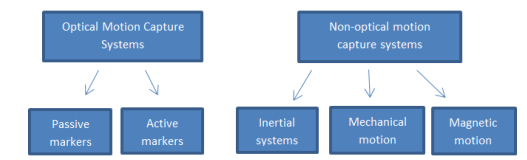
\includegraphics[width=0.7\textwidth]{figures/Mocap.png}
	\caption{MoCap systems Hierarchy}
\end{figure}

Motion analysis data collection protocols, measurement precision, and data reduction models have all been developed to meet the needs of their respective settings. Sport assessments, for example, necessitate higher data acquisition rates due to higher velocities than normal walking. Furthermore, real-time tracking is required for a realistic user experience, so time lag should be kept to a minimum. Years of technological advancement have resulted in numerous systems that can be classified as optical and non-optical, where non-optical category contains mechanical, magnetic, or inertial trackers. The human body is frequently viewed as a network of rigid links connected by joints. Human body parts are not rigid structures, but they are commonly treated as such during human motion studies. 
\pagebreak
\subsubsection{Optical Motion Capture}

\begin{figure}[h]
	\centering
	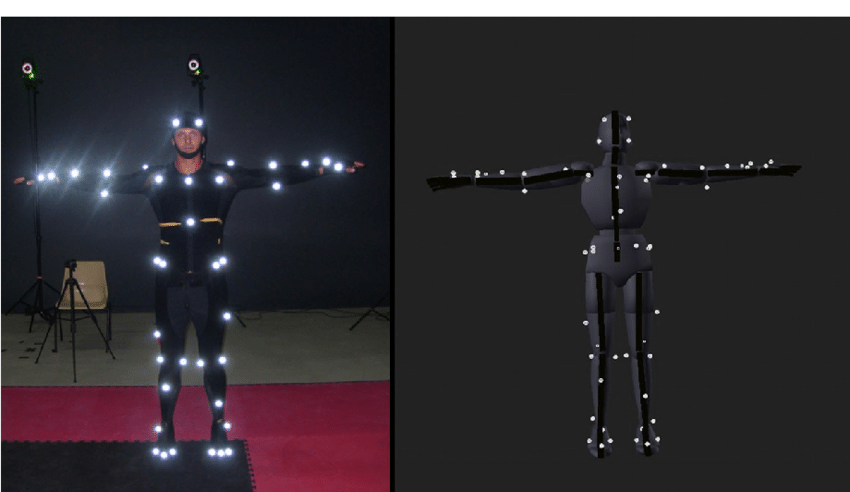
\includegraphics[width=0.6\textwidth]{figures/background/Optical.png}
	\caption{\href{https://www.researchgate.net/profile/Jacek-Hordyj/publication/283152771/figure/fig1/AS:669997391159296@1536751234023/Actor-wearing-suit-adjusted-for-optical-motion-capture-on-the-left-Virtual-model.png}
	{Optical Motion Capture suit}}
\end{figure}

Multiple high-speed cameras   \cite{Optical Motion Capture: Theory and Implementation,MOTION CAPTURE TO BUILD A FOUNDATION FOR A COMPUTER-CONTROLLED INSTRUMENT BY STUDY OF CLASSICAL GUITAR PERFORMANCE} or video cameras are used in optical motion capture systems to triangulate the position of each marker on the actor. This method involves using a series of synchronized cameras to capture markers placed in strategic locations on the body. More specifically, a number of synchronized cameras, an image acquisition system, a capturing area, and a special suit with markers are all required for the implementation of an optical motion capture system.The positions of the markers on the suit are designed to cover the necessary body parts.\\

Passive optical marker systems employ a variety of highly reflective markers of varying sizes that reflect light back to cameras. These markers can be velcroed to a body suit or applied directly to the skin. A ring of visible red, near red, or infrared strobe light emitting diodes (LEDs) around the camera lens generates the reflected light. The cameras' light sensitivity can be adjusted to reject other sources of light. Passive markers have the advantage of not requiring a power source such as batteries, wiring, or other electronic devices. The downside is that to the cameras, all of the markings appear to be the same. This means that if many markers are occluded and subsequently reappear in camera view, the cameras are unable to distinguish between them.\\

Active optical marker systems employ powered LEDs as markers.
Unlike passive markers, which reflect light back to cameras, these markers emit their own visible red or infrared light. These markers, like passive markers, can be adhered directly to the skin or velcroed to a body suit. The advantages of active markers are that each LED modulates and emits a unique frequency, resulting in each marker being uniquely identified. The disadvantage is that each LED must be powered, which necessitates the use of wires and related devices like batteries and circuit boards.
 
\pagebreak
\subsubsection{Non-Optical Motion Capture}
\subsubsection*{Inertial Motion Capture}
\begin{figure}[h]
	\centering
	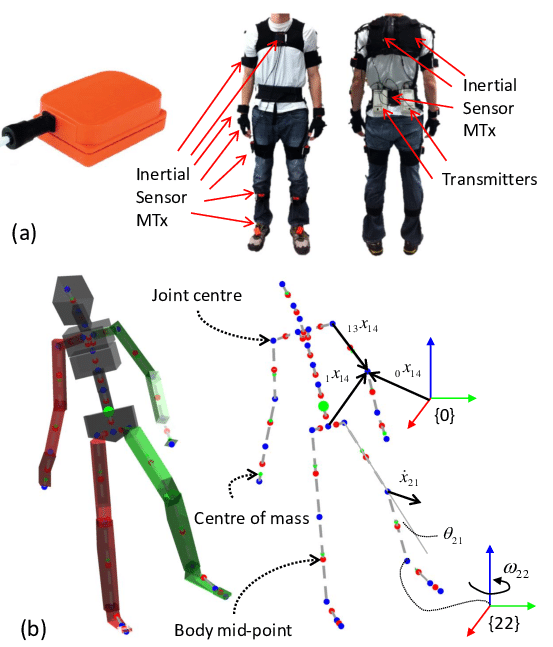
\includegraphics[width=0.4\textwidth]{figures/background/Inertial.png}
	\caption{\href{https://www.researchgate.net/profile/Matthew-Field-6/publication/257308000/figure/fig1/AS:613448983531582@1523269043700/a-The-inertial-sensor-MTx-left-14-and-positioning-of-the-sensors-and-wireless.png}
	{Inertial sensor suit}}
\end{figure}

Inertial sensors \cite{Kalman Filtering for Sensor Fusionin a Human Tracking System} rely on the property of bodies to maintain constant translational and rotational velocity unless perturbed by forces or torques. The vestibular system is a biological 3D inertial sensor located in the inner ear. It can detect both angular motion and linear acceleration of the head. The vestibular system is critical for maintaining eye balance and stabilization in relation to the environment. Advances in miniaturized and micro-machined sensor technologies, particularly silicon accelerometers and rate sensors, have made practical inertial tracking possible. A rate gyroscope measures angular velocity and provides the change in angle with respect to an initially known angle when integrated over time. Accelerations, including gravitational acceleration g, are measured by an accelerometer.\\

If the sensor's angle with respect to the vertical is known, the gravity component can be removed and velocity and position can be calculated using numerical integration. If no compensation is used, the noise and bias errors associated with small and inexpensive sensors make tracking orientation and position for long periods of time impractical. Drift and other errors can be reduced by combining signals from inertial sensors with those from aiding/complementary sensors and using knowledge about their signal characteristics.

\subsubsection*{Mechanical Motion Capture}

\begin{figure}[h]
	\centering
	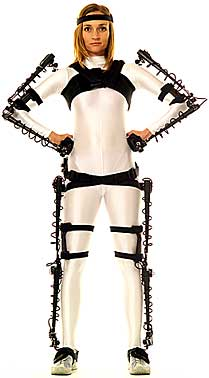
\includegraphics[width=0.3\textwidth]{figures/background/Mechanical.png}
	\captionsetup{labelformat=empty}
	\caption{\href{https://metamotion.com/images/gypsy4_standing.jpg}
	{Mechanical mocap suit}}
\end{figure}

Because of the external structure \cite{MOTION CAPTURE TO BUILD A FOUNDATION FOR A COMPUTER-CONTROLLED INSTRUMENT BY STUDY OF CLASSICAL GUITAR PERFORMANCE} that is attached to the performer, mechanical motion capture systems are also known as exoskeleton motion capture systems. These structures, which are typically made of rigid metal or plastic, have articulated joints with potentiometers that directly measure a performer's joint angles as he or she moves. One of the primary benefits of this direct measurement system is the absence of the need for cameras or other sensors. The system's main drawbacks are that the performer is restricted to the degrees of freedom of the structure and that the location of the sensor placement is fixed. If the performer attempts to move beyond the system's degrees of freedom, the structure may be damaged or broken.

\pagebreak

\subsubsection*{Magnetic Motion Capture}

\begin{figure}[h]
	\centering
	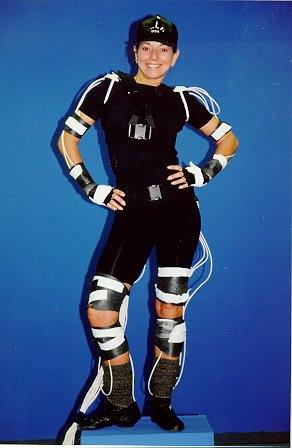
\includegraphics[width=0.3\textwidth]{figures/background/Magnetic.png}
	\captionsetup{labelformat=empty}
	\caption{\href{https://www.researchgate.net/profile/Jessica-Hodgins-2/publication/2359279/figure/fig4/AS:669524957331457@1536638597171/A-performer-wearing-a-motion-capture-apparatus-The-device-shown-is-a-full-body-magnetic.ppm}
	{Magnetic mocap suit}}
\end{figure}

Magnetic motion capture systems \cite{MOTION CAPTURE TO BUILD A FOUNDATION FOR A COMPUTER-CONTROLLED INSTRUMENT BY STUDY OF CLASSICAL GUITAR PERFORMANCE} work by measuring the low-frequency magnetic field produced by a source transmitter and relaying it to a receiver. Each transmitter and receiver have three orthogonal coils that measure magnetic flux between them and calculate the position and orientation of each sensor. One of the key advantages of these systems is that instead of the more conventional three degrees of position, each sensor transmitter/receiver pair may capture both orientation and position. However, sensors in the system, are susceptible to environmental metal, magnetic fields, and electrical sources such as rebar walls and floors, lights, cables, monitors, and computers. Shielding equipment and wiring requires special care. Despite their high accuracy, the sensors become nonlinear at the extremes of their range. 
\subsection{Related Work}
\subsection{First Approach, with GAN's}
\subsubsection{Dataset}
\subsubsection{Theory}
\subsubsection{Cons and Pros of this idea}
\newpage
\section{Requirements}
\subsection{Hardware}
\subsection{Input requirements}
\subsection{Application's UI}
\newpage
\section{Implementation}
\subsection{Mocap Dataset Augmentation using pretrained models}
\subsubsection{Dataset Augmentation}
\subsubsection{Available Pretrained Models}
\subsubsection{Alpha-pose model}
\subsubsection{Orientation and location estimation}
\subsection{Animator Tools}
\subsubsection{Fast BVH Editing}
\subsubsection{BVH Filtering}
\subsection{Windows Application}
\subsubsection{Tkinter library}
\subsubsection{Construction of the Application }
\newpage
\section{Evaluation}
\subsection{Algorithm Accuracy}
\subsection{Comparing Result}
\newpage
\section{Discussion}
\subsection{Drawbacks of our Work}
\subsection{Future Approaches}
\newpage
\begin{thebibliography}{9}

\bibitem{Efficient Content-Based Retrieval of Motion Capture Data}
M{\"u}ller, Meinard and R{\"o}der, Tido and Clausen, Michael ACM SIGGRAPH 2005 Papers 677--685\\

\bibitem{Exploiting temporal information for 3D pose estimation}
Rayat Imtiaz Hossain, Mir, and James J. Little. "Exploiting temporal information for 3D pose estimation." arXiv e-prints (2017): arXiv-1711.\\

\bibitem{3D Human Pose Estimation from Deep Multi-View 2D Pose}
Schwarcz, Steven, and Thomas Pollard. "3d human pose estimation from deep multi-view 2d pose." 2018 24th International Conference on Pattern Recognition (ICPR). IEEE, 2018.\\

\bibitem{3D Human Pose Estimation Using Convolutional Neural Networks with 2D Pose Information}
Park, Sungheon, Jihye Hwang, and Nojun Kwak. "3d human pose estimation using convolutional neural networks with 2d pose information." European Conference on Computer Vision. Springer, Cham, 2016.\\

\bibitem{Review on Motion Capture Technology}
Rahul, M. "Review on motion capture technology." Global Journal of Computer Science and Technology (2018).\\

\bibitem{Optical Motion Capture: Theory and Implementation}
Guerra-Filho, Gutemberg. "Optical Motion Capture: Theory and Implementation." RITA 12.2 (2005): 61-90.\\

\bibitem{Kalman Filtering for Sensor Fusionin a Human Tracking System}
Corrales Ramón, Juan Antonio, Francisco A. Candelas-Herías, and Fernando Torres. Kalman filtering for sensor fusion in a human tracking system. Intech, 2010.\\

\bibitem{MOTION CAPTURE TO BUILD A FOUNDATION FOR A COMPUTER-CONTROLLED INSTRUMENT BY STUDY OF CLASSICAL GUITAR PERFORMANCE}
 Norton, Jonathan Carey. Motion capture to build a foundation for a computer-controlled instrument by study of classical guitar performance. Stanford University, 2008.\\
 
\bibitem{Deep Learning}
https://www.deeplearningbook.org/\\

\bibitem{ANIMGAN: A SPATIOTEMPORALLY-CONDITIONED GENERATIVE ADVERSARIAL NETWORK FOR CHARACTER ANIMATION}
Mirzaei, Maryam Sadat, et al. "Animgan: A spatiotemporally-conditioned generative adversarial network for character animation." 2020 IEEE International Conference on Image Processing (ICIP). IEEE, 2020.\\

\bibitem{3D Human Pose Estimation = 2D Pose Estimation + Matching}
Chen, Ching-Hang, and Deva Ramanan. "3d human pose estimation= 2d pose estimation+ matching." Proceedings of the IEEE Conference on Computer Vision and Pattern Recognition. 2017.\\

\bibitem{The importance of the loss function in option valuation}
Christoffersen, Peter, and Kris Jacobs. "The importance of the loss function in option valuation." Journal of Financial Economics 72.2 (2004): 291-318.\\

\bibitem{Human3.6M}
Ionescu, Catalin, et al. "Human3. 6m: Large scale datasets and predictive methods for 3d human sensing in natural environments." IEEE transactions on pattern analysis and machine intelligence 36.7 (2013): 1325-1339.\\

\bibitem{OpenPose}
Cao, Zhe, et al. "Realtime multi-person 2d pose estimation using part affinity fields." Proceedings of the IEEE conference on computer vision and pattern recognition. 2017.\\

\bibitem{HrNet}
Sun, Ke, et al. "Deep high-resolution representation learning for human pose estimation." Proceedings of the IEEE/CVF Conference on Computer Vision and Pattern Recognition. 2019.\\

\bibitem{AlphaPose}
Fang, Hao-Shu, et al. "Rmpe: Regional multi-person pose estimation." Proceedings of the IEEE international conference on computer vision. 2017.\\

\bibitem{ANIMGAN}
Mirzaei, Maryam Sadat, et al. "Animgan: A spatiotemporally-conditioned generative adversarial network for character animation." 2020 IEEE International Conference on Image Processing (ICIP). IEEE, 2020.\\

\bibitem{Human Action Generation with Generative
Adversarial Networks}
Kiasari, Mohammad Ahangar, Dennis Singh Moirangthem, and Minho Lee. "Human action generation with generative adversarial networks." arXiv preprint arXiv:1805.10416 (2018).\\

\bibitem{SPPE}
Zhang, Feng, Xiatian Zhu, and Chen Wang. "Single Person Pose Estimation: A Survey." arXiv preprint arXiv:2109.10056 (2021).\\

\bibitem{YOLO-Pose}
Maji, Debapriya, et al. "YOLO-Pose: Enhancing YOLO for Multi Person Pose Estimation Using Object Keypoint Similarity Loss." arXiv preprint arXiv:2204.06806 (2022).\\

\bibitem{YOLOv3}
Redmon J, Farhadi A, "YOLOv3: an Incremental Improvement," https://arxiv.org/
abs/1804.02767, 2018.

\bibitem{HourGlass}
Newell, Alejandro, Kaiyu Yang, and Jia Deng. "Stacked hourglass networks for human pose estimation." European conference on computer vision. Springer, Cham, 2016.

\bibitem{Attention Mechanism Exploits Temporal Contexts: Real-time 3D Human Pose Reconstruction}
Liu, Ruixu, et al. "Attention mechanism exploits temporal contexts: Real-time 3d human pose reconstruction." Proceedings of the IEEE/CVF Conference on Computer Vision and Pattern Recognition. 2020.\\

\bibitem{3D human pose estimation in video with temporal convolutions and semi-supervised training}
Pavllo, Dario, et al. "3d human pose estimation in video with temporal convolutions and semi-supervised training." Proceedings of the IEEE/CVF Conference on Computer Vision and Pattern Recognition. 2019.\\

\bibitem{Mean Filtering}
Chandrinos, Aristeidis. "The Challenge of Predicting OAG Progression from the Initial Visual Field Test." Signal 4: 6.\\

\bibitem{Gaussian Filtering}
Ramamurthy, Arjun. "An All Digital Implementation of Constant Envelope: Bandwidth Efficient GMSK Modem using Advanced Digital Signal Processing Techniques." Wireless personal communications 52.1 (2010): 133-146.\\

\bibitem{Butterworth Filtering}
Cuadrado, Javier, Florian Michaud, Urbano Lugrís, and Manuel Pérez Soto. "Using accelerometer data to tune the parameters of an extended kalman filter for optical motion capture: Preliminary application to gait analysis." Sensors 21, no. 2 (2021): 427.\\

\bibitem{Tkinter 1}
Lundh, Fredrik. "An introduction to tkinter." URL: www. pythonware. com/library/tkinter/introduction/index. htm (1999).\\

\bibitem{Tkinter 2}
Grayson, John E. Python and Tkinter programming. Manning Publications Co. Greenwich, 2000.\\

\bibitem{MS COCO}
Lin, Tsung-Yi, Michael Maire, Serge Belongie, James Hays, Pietro Perona, Deva Ramanan, Piotr Dollár, and C. Lawrence Zitnick. "Microsoft coco: Common objects in context." In European conference on computer vision, pp. 740-755. Springer, Cham, 2014.\\

\bibitem{AP}
https://jonathan-hui.medium.com/map-mean-average-precision-for-object-detection-45c121a31173\\

\bibitem{OCHuman}
Zhang, Song-Hai, Ruilong Li, Xin Dong, Paul Rosin, Zixi Cai, Xi Han, Dingcheng Yang, Haozhi Huang, and Shi-Min Hu. "Pose2seg: Detection free human instance segmentation." In Proceedings of the IEEE/CVF Conference on Computer Vision and Pattern Recognition, pp. 889-898. 2019.\\

\end{thebibliography}

 
% \section{Introduction} \label{ch1}
% \input{sources/1_introduction.tex} 

\label{EndOfText}

\label{endOfDoc}

\end{document}
